\chapter{Resultados}

\section{Software Composer}
Como primeiro resultado de desenvolvimento de software em computação musical e artística foi consolidado o software Composer. Tal software web, desenvolvido em Ruby on Rails, tem como objetivo a composição de uma música através de partes cortadas de uma mesma música. O usuário irá selecionar essas partes na ordem que desejar e no final o software construirá uma música de acordo com a ordem selecionada pelo usuário. Segue abaixo a tela inicial da aplicação:

\begin{figure}[h!]
        \centering
        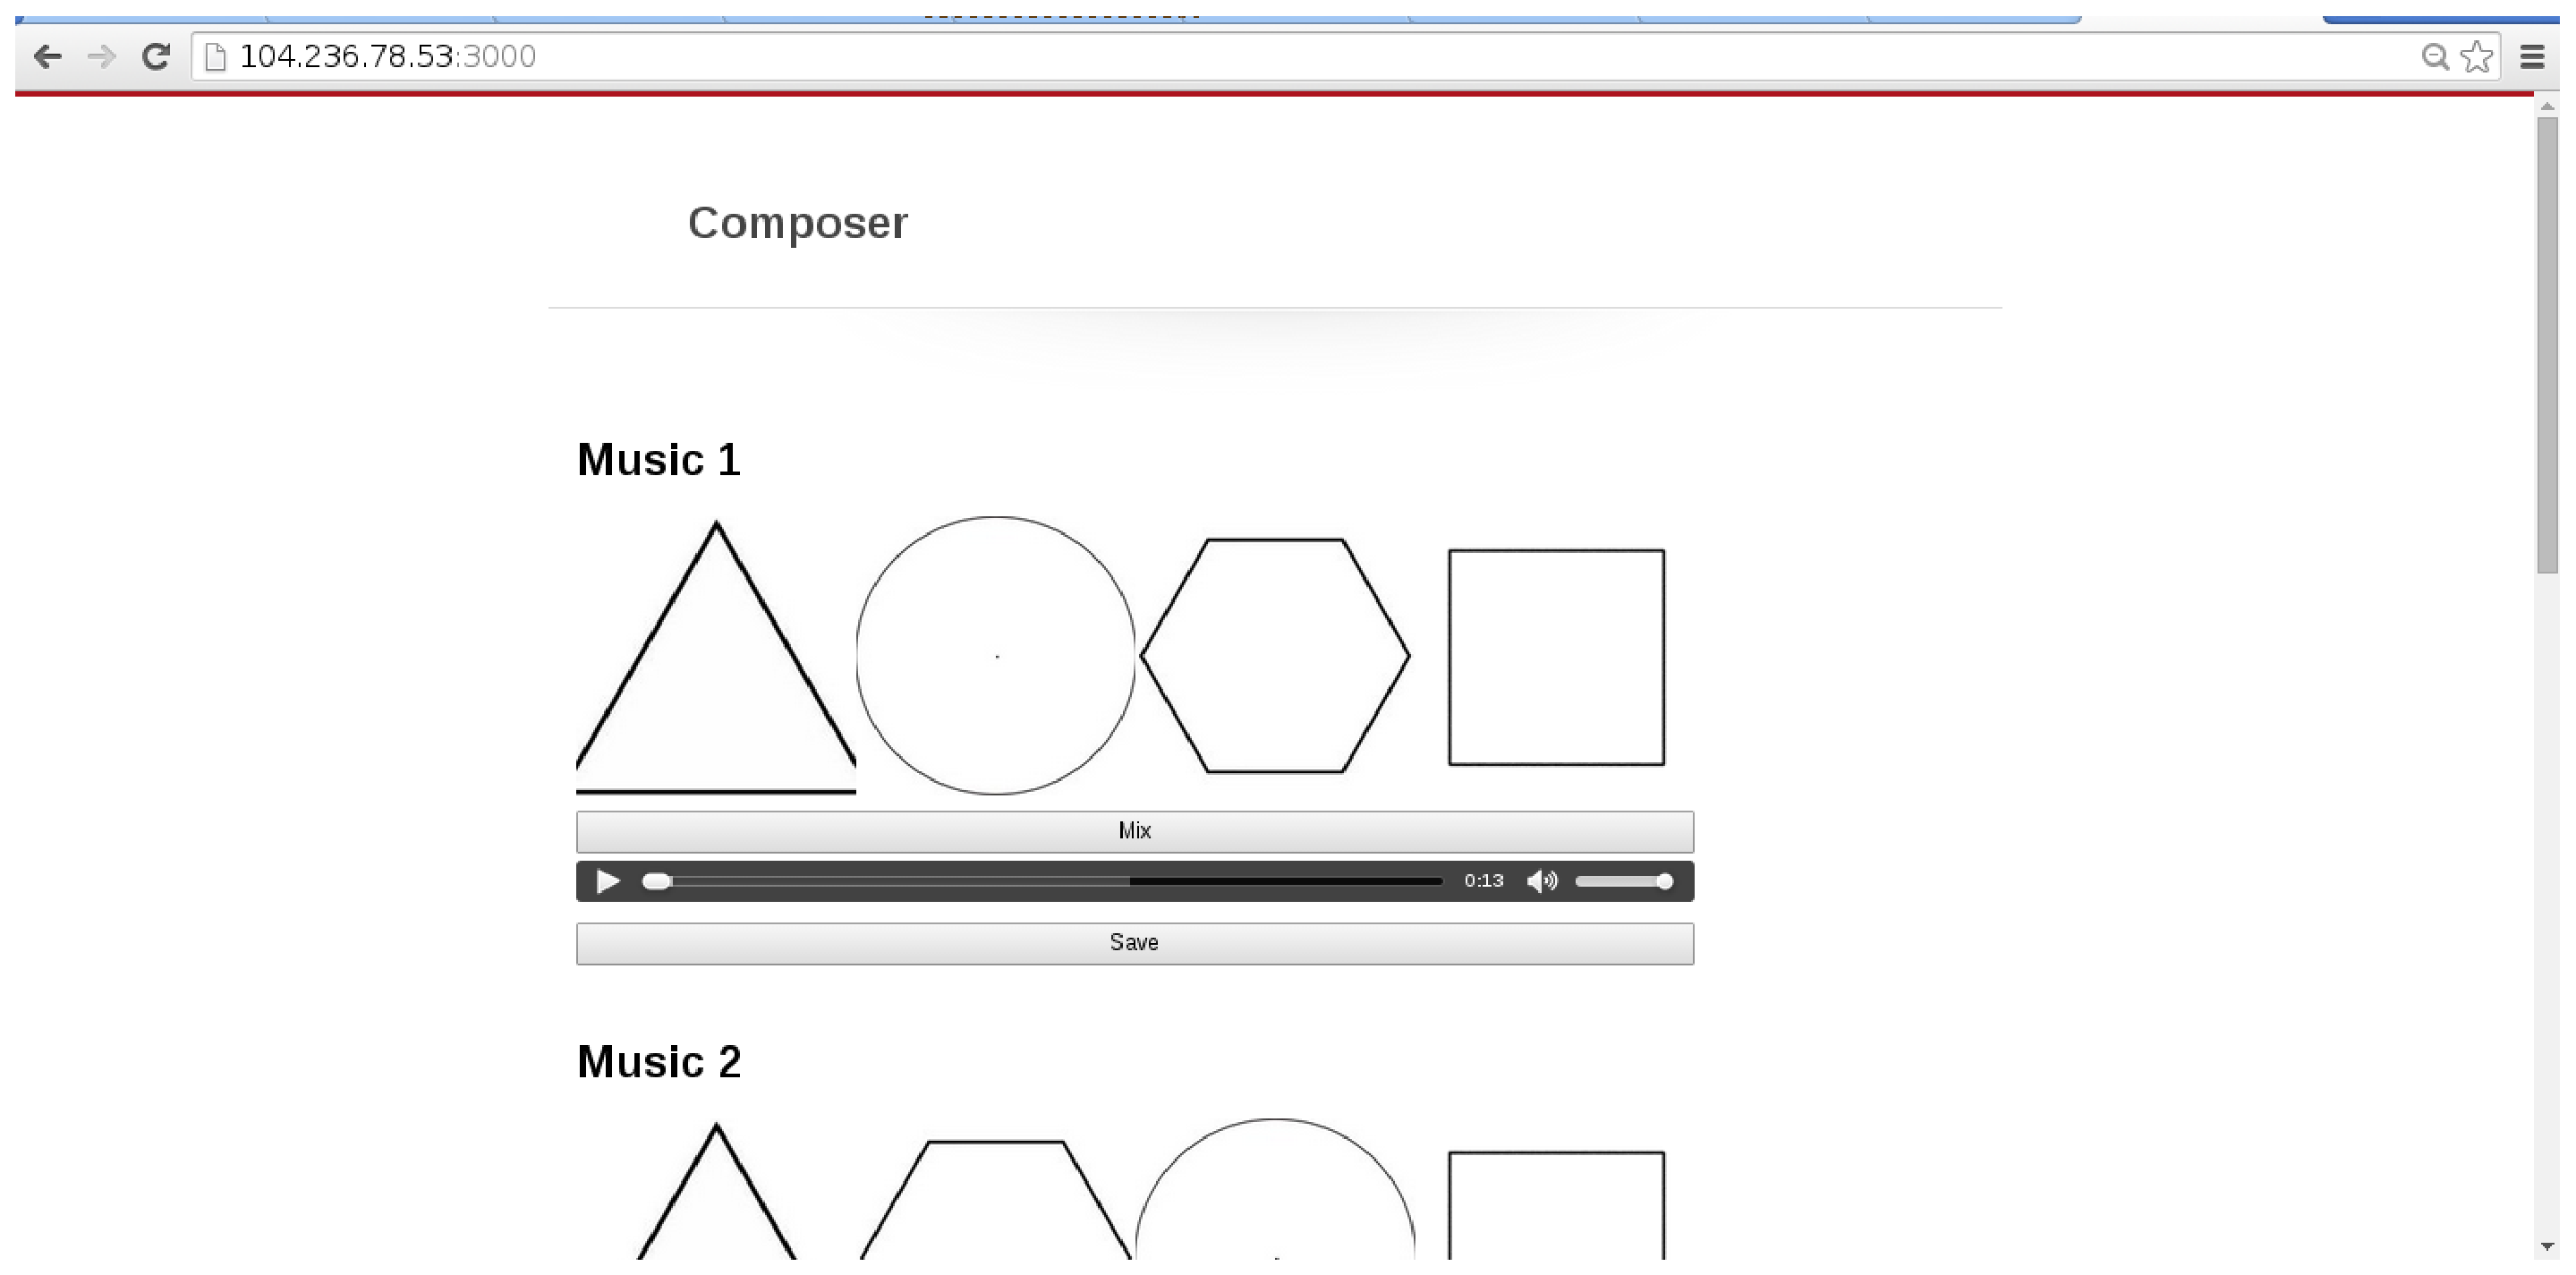
\includegraphics[width=0.9\textwidth]{figuras/composer_1.eps}
        \caption{Tela inicial do software composer}
        \label{fig:cronograma}
\end{figure}

Atrás de cada figura há um campo numérico para a inserção da ordem de cada faixa musical. Ao colocar a ordem, o usuário irá pressionar o botão $mix$ e em seguida serão passados os parâmetros de ordem na url via método GET para a classe controladora. Em seguida esses parâmetros estarão disponíveis no método da controladora $index$. Segue uma parte do código desse método para a composição de uma música:

\begin{lstlisting}
  if params[:"Heitor_6a"] != nil
    files_to_append = ["/var/www/html/"+formation_audio.key("1")+".wav", 
      "/var/www/html/"+formation_audio.key("2")+".wav",
       "/var/www/html/"+
      formation_audio.key("3")+".wav",
       "/var/www/html/"+formation_audio.key("4")+".wav"]
    samples_per_buffer = 4096
    
    File.open('/var/www/html/report.txt', 'a+') { |file| 
    	file.write("\n"+Time.now.day.to_s+'-'+Time.now.month.to_s+'-'
    		+Time.now.year.to_s+'_'+Time.now.hour.to_s+':'+
    		Time.now.min.to_s+':'+Time.now.sec.to_s+" - \t"+
    		formation_audio.key("1")+', '+formation_audio.key("2")+', 
    		'+formation_audio.key("3")+', 
    		'+formation_audio.key("4")) }    

    Writer.new("/var/www/html/audioHeitor.wav", 
    	Format.new(:stereo, :pcm_16, 44100)) do |writer|
      files_to_append.each do |file_name|
        Reader.new(file_name).
        each_buffer(samples_per_buffer) do |buffer|
          writer.write(buffer)
        end
      end
    end
    end
\end{lstlisting}

O código acima é formado por 3 blocos principais. O primeiro bloco se refere a ordem em que as partes das músicas serão montadas através de um vetor de $strings$ contendo os locais de cada parte. O segundo bloco se refere a escrita de um $log$ que conterá os registros de cada usuário relativos a ordem escolhida das partes musicais. O terceiro bloco é a montagem das partes musicais num arquivo .wav.

Dado a música montada, o usuário poderá baixar ela segundo a imagem abaixo:

\begin{figure}[h!]
        \centering
        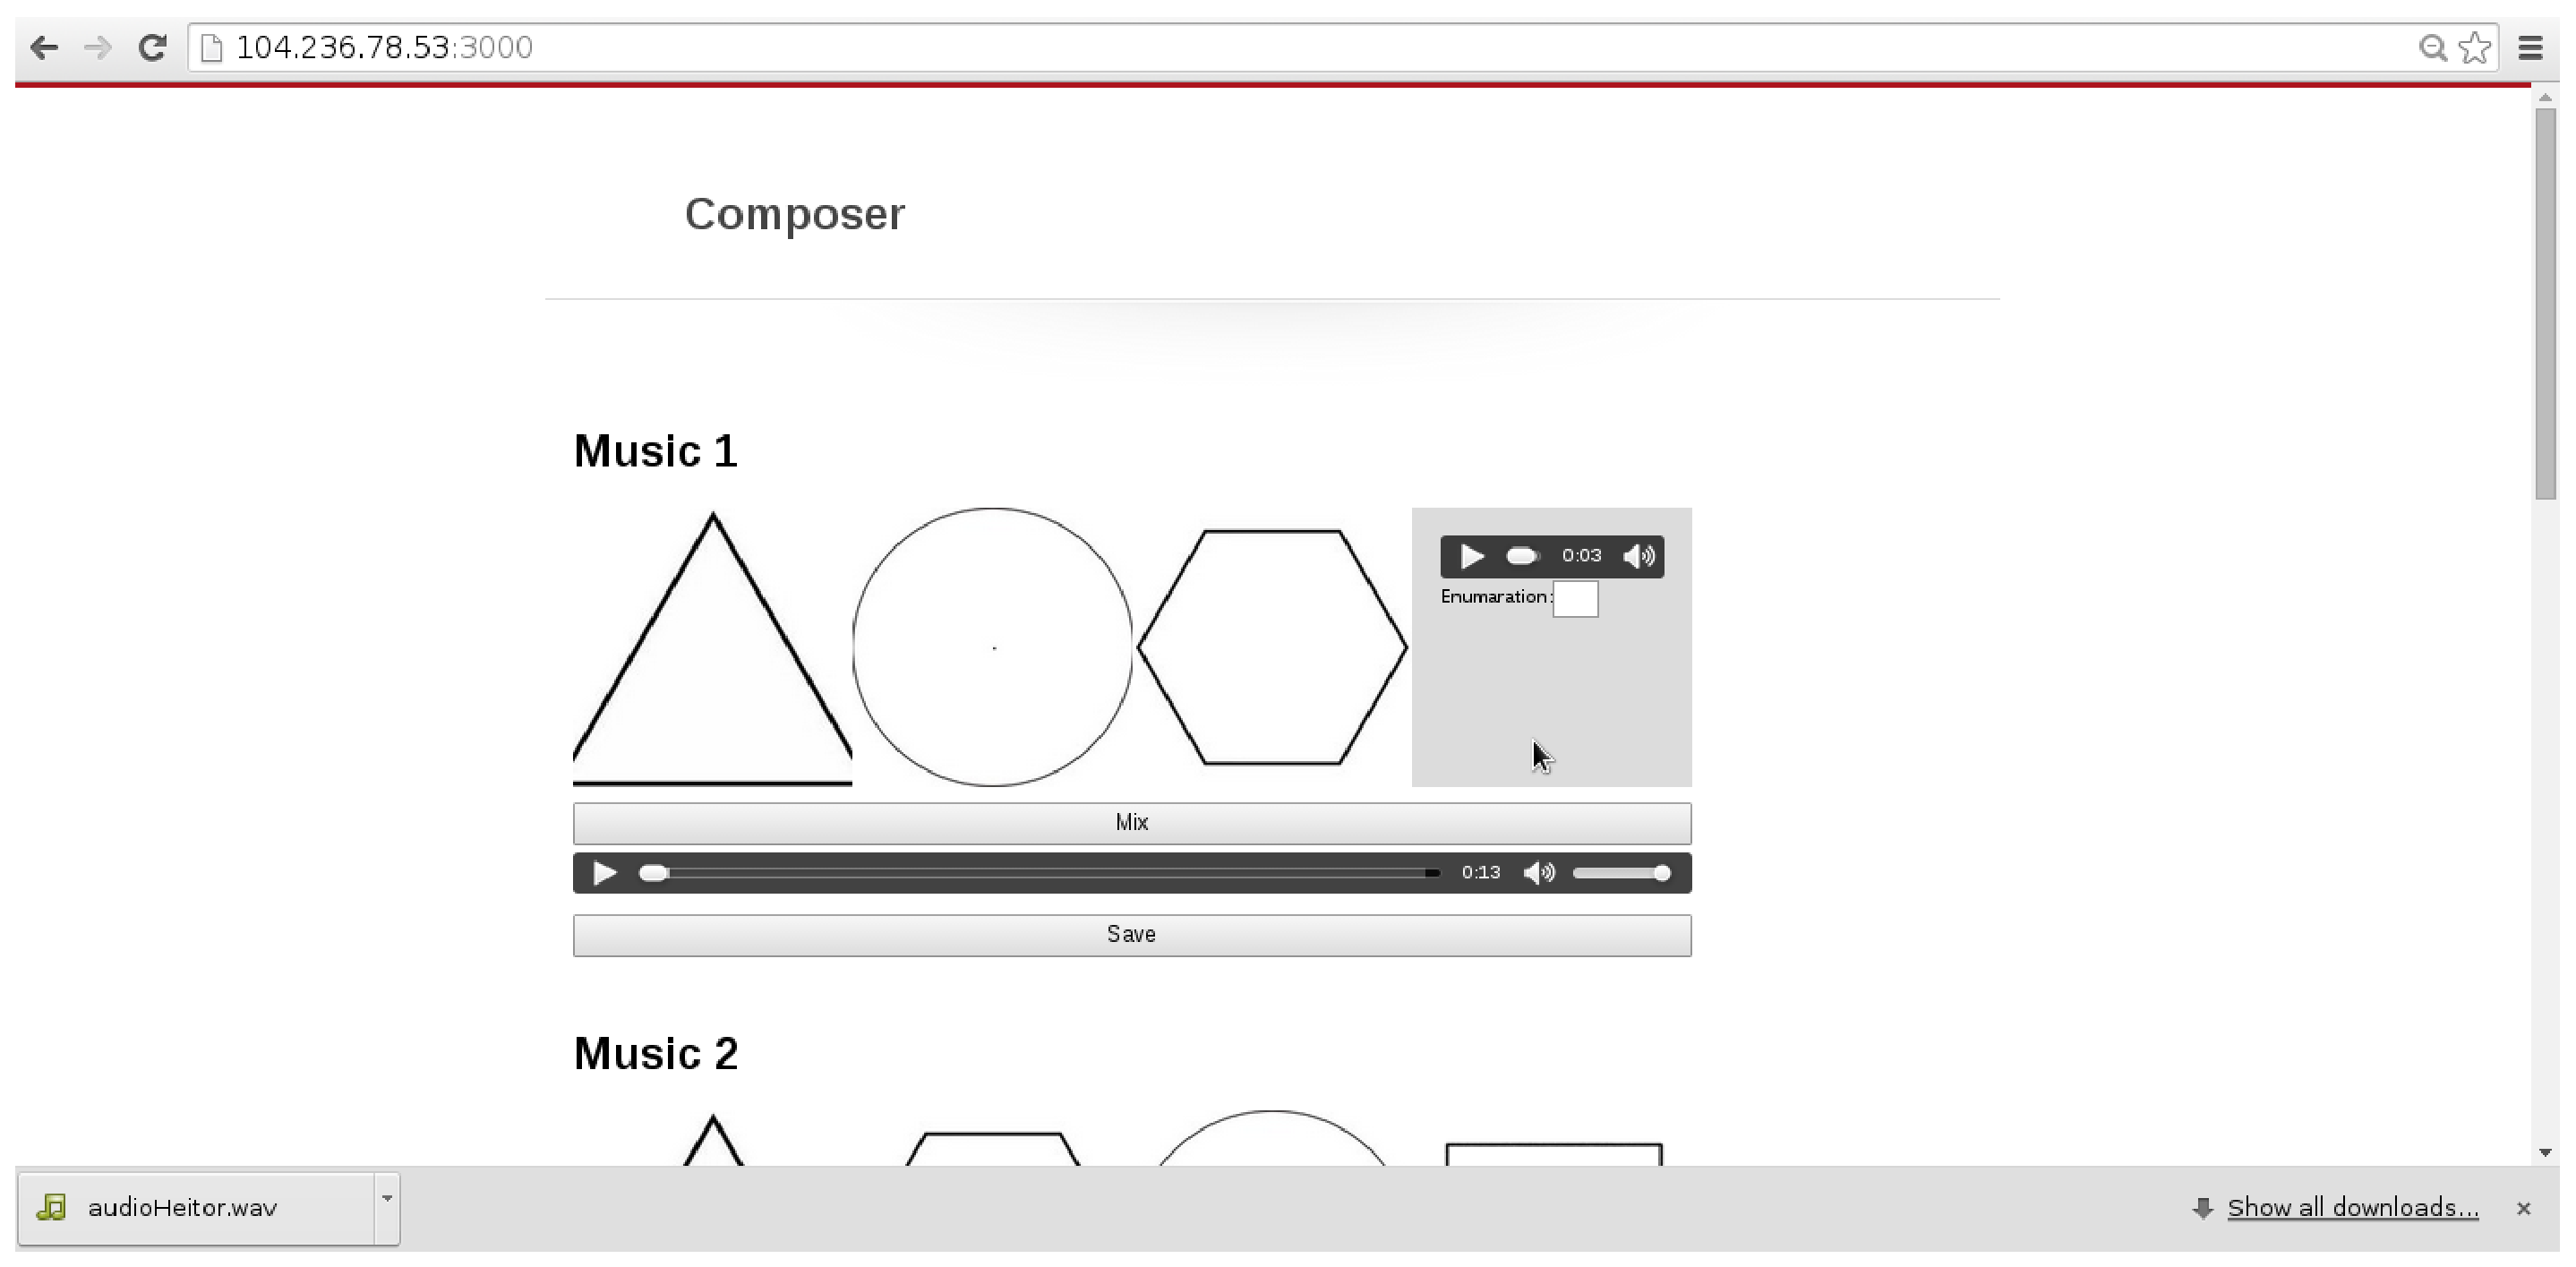
\includegraphics[width=0.9\textwidth]{figuras/composer_2.eps}
        \caption{Download de música do software composer}
        \label{fig:cronograma}
\end{figure}

Para tal função o software requisita a função $edit$ da controladora que possui o seguinte código:
\begin{lstlisting}
def edit
    if @friend == Friend.all[0]
      send_file '/var/www/html/audioHeitor.wav', 
      :type=>"application/wav", :x_sendfile=>true  
    end
    if @friend == Friend.all[4]
      send_file '/var/www/html/audioCseko.wav',
       :type=>"application/wav", :x_sendfile=>true  
    end
    if @friend == Friend.all[8]
      send_file '/var/www/html/audioSeincman.wav', 
      :type=>"application/wav", :x_sendfile=>true  
    end
    if @friend == Friend.all[12]
      send_file '/var/www/html/audioZampronha.wav', 
      :type=>"application/wav", :x_sendfile=>true  
    end
    
  end
\end{lstlisting}

Para cada $@friend$ a controladora irá mandar um arquivo de música montado de acordo com os parâmetros do usuário. Para mais detalhes de projeto o código os mesmos podem ser encontrados no repositório git: https://github.com/josepedro/composer.

\section{Snake Chords}

Como segundo resultado de desenvolvimento de software em computação musical e artística foi consolidado o software Snake Chords. Tal software $mobile$, desenvolvido em Java/Android, é um jogo cujo objetivo é o usuário movimentar uma serpente para pontuar através de reconhecimento de padrões harmônicos num instrumento musical, por exemplo, violão. O usuário irá tocar acordes do instrumento musical e a serpente irá se mover de acordo com os acordes tocados. Segue abaixo a tela inicial da aplicação:

\begin{figure}[h!]
        \centering
        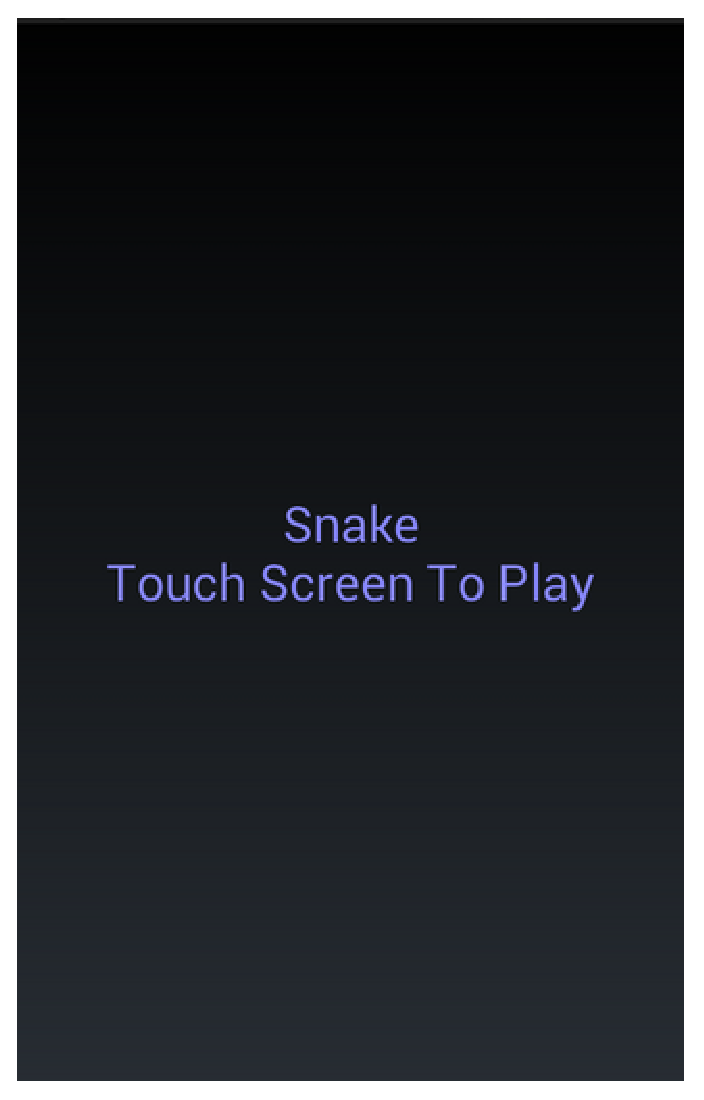
\includegraphics[width=0.3\textwidth]{figuras/snake_1.eps}
        \caption{Tela inicial do software Snake Chords}
        \label{fig:cronograma}
\end{figure}

\newpage
Ao tocar na tela o usuário começa a controlar a serpente no intuito de capturar os círculos amerelos que aparecem de forma aleatória. A seguinte imagem mostra a tela seguinte com a interação do usuário com a serpente em movimento:
\begin{figure}[h!]
        \centering
        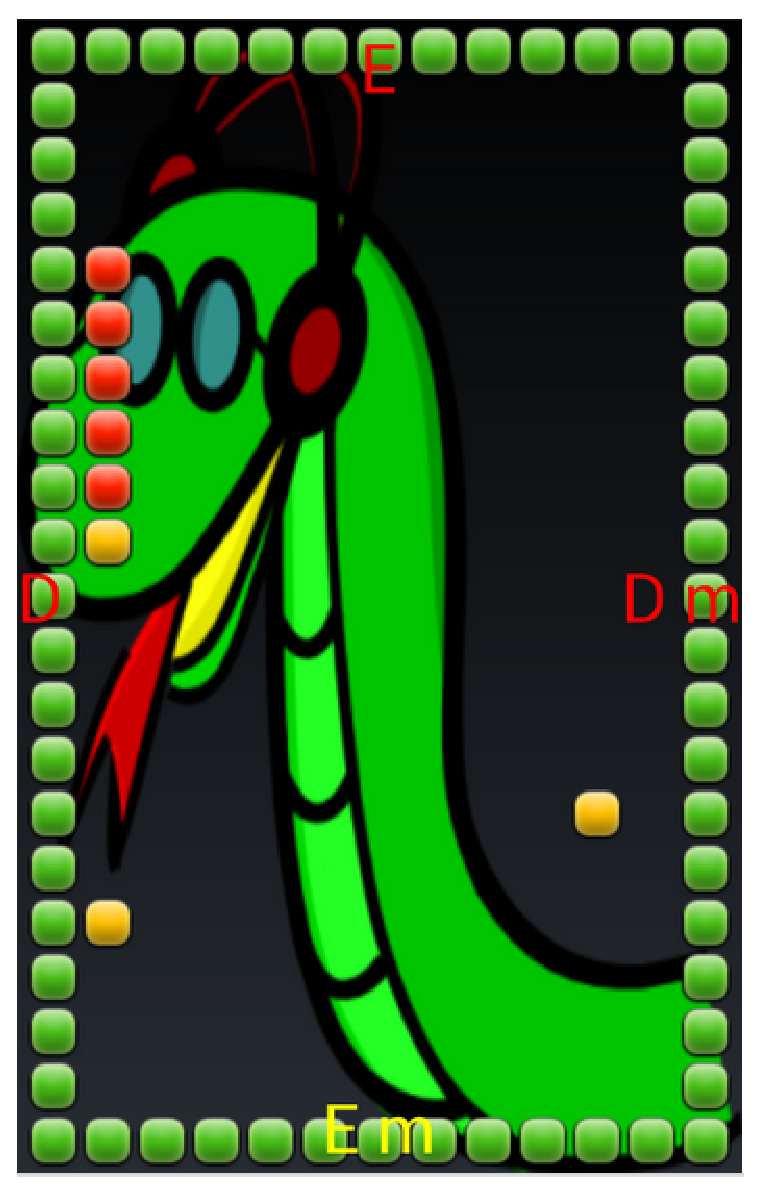
\includegraphics[width=0.3\textwidth]{figuras/snake_2.eps}
        \caption{Software Snake Chords}
        \label{fig:cronograma}
\end{figure}

No que tange a implementação do mesmo, o sistema possui 5 classes. A classe principal é a $Snake.java$. Segue uma parte do código da mesma:
\begin{lstlisting}
  @Override
    public void onCreate(Bundle savedInstanceState) {
        super.onCreate(savedInstanceState);
        setContentView(R.layout.snake_layout);
        myfft = new MyFFT();
        asyncTaskChords = new RecordingAndSetChord();
        asyncTaskChords.execute();
        mSnakeView = (SnakeView) findViewById(R.id.snake);
        mSnakeView.setDependentViews((TextView) 
        	findViewById(R.id.text),
                findViewById(R.id.arrowContainer)
                , findViewById(R.id.background));
        if (savedInstanceState == null) {
            // We were just launched -- set up a new game
            mSnakeView.setMode(SnakeView.READY);
        } else {
            // We are being restored
            Bundle map = savedInstanceState.
            getBundle(ICICLE_KEY);
            if (map != null) {
                mSnakeView.restoreState(map);
            } else {
                mSnakeView.setMode(SnakeView.PAUSE);
            }
        }

        mSnakeView.setOnTouchListener(new OnTouchListener() {
            @Override
            public boolean onTouch(View v, MotionEvent event) {
                if (mSnakeView.getGameState() == SnakeView.RUNNING) {
                    // Normalize x,y between 0 and 1
                    float x = event.getX() / v.getWidth();
                    float y = event.getY() / v.getHeight();
                    // Direction will be [0,1,2,3] depending on quadrant
                    int direction = 0;
                    direction = (x > y) ? 1 : 0;
                    direction |= (x > 1 - y) ? 2 : 0;
                } else {
                    mSnakeView.moveSnake(MOVE_UP);
                }
                return false;
            }
        });
    }
\end{lstlisting}

O código acima possui dois blocos principais. O primeiro bloco diz respeito às instâncias iniciais do método do ciclo de vida Android $onCreate$. É instanciado elementos de $view$ em $setContentView(R.layout.snake_layout)$, classe para reconhecimento de padrões harmônicos $myfft = new MyFFT()$ e classe para execução de $threads$ de gravação de som em $asyncTaskChords = new RecordingAndSetChord()$. Ao final o contexto é guardado no método do ciclo de vida do Android $savedInstanceState$ para recomeçar o jogo de onde parou toda vez que haver interrupção. O outro bloco relativo ao $Listener$ $mSnakeView.setOnTouchListener(new OnTouchListener()$ diz respeito a inicialização do jogo depois do toque na tela. Para mais detalhes de projeto o código os mesmos podem ser encontrados no repositório git: https://github.com/josepedro/snake\_enchanter.

